\subsubsectionwithauthor[author={Mika Landeck},email={mika.landeck@fau.de}]{Aufgabe 2: Minimale DEAs}

	
\paragraph{(a)}
		Allgemein eignet sich für die Prüfung der Minimalität eines DEA das sogenannte \glqq Tabellenfüllverfahren\grqq (im Englischen \textit{table filling algorithm} oder \textit{table filling method}). Dabei wird eine Tabelle (mit allen erreichbaren Zuständen) aufgestellt, in der nicht äquivalente Zustandspaare gekennzeichnet werden. In dieser Tabelle wird zunächst in allen Zellen, deren zugehöriges Zustandspaar einen Endzustand und einen Nicht-Endzustand enthält, ein $X_0$ notiert - diese Paare können sicher nicht äquivalent sein.\\		
		Nun wird versucht, von den übrigen Zellen aus die bereits gefüllten Zellen durch Über- gänge aus dem Automaten zu erreichen. Dies wird so lange wiederholt, bis sich keine Änderungen in der treppenförmigen Tabelle mehr ergeben. Wenn dann noch Zellen ungefüllt bleiben, bedeutet das, dass die Zustände des entsprechenden Zustandspaares äquivalent sind.\\
		Alle zueinander äquivalenten Zustände liegen dann in einer Äquivalenzklasse, die nicht äquivalenten Zustände bilden jeweils eine eigene Äquivalenzklasse. Diese Äquivalenz- klassen bilden die Zustände des minimierten DEA.
		
		Für den ersten DEA bleibt keine Zelle der Tabelle ungefüllt, was bedeutet, dass hier keine äquivalenten Zustände vorliegen. Da jeder Zustand erreichbar ist, ist der Automat also bereits minimal:
	
	\includegraphics[scale=0.75]{Tabellenfüllverfahren2.png}
	
	\begin{tabular}{c|c|c|l}
		\textbf{Zustandspaar} & \textbf{a} & \textbf{b} & \textbf{Erläuterung} \\
		\hline
		(2,1)                 & (0,1)      & (3,3)      & Eingabe b: (3,3) führt zu X0. Ergänze X1. \\
		\hline
		(2,0)                 & (0,1)      & (2,1)      & Eingabe b: (2,1) führt zu X1. Ergänze X2. \\
		\hline
		(1,0)                 & (1,1)      & (2,3)      & Eingabe b: (2,3) führt zu X0. Ergänze X3. \\
	\end{tabular} \\

\paragraph{(b)}
		Eine Zeugentabelle zum Automaten zeigt, dass der Zustand 1 nicht erreichbar ist:

		\begin{tabular}{l|c|c|c|c}
			\textbf{Zustand} & \textbf{0} & \textbf{1} & \textbf{2} & \textbf{3} \\
			\hline
			\textbf{Zeuge} & $\epsilon$ & $-$ & $a$ & $aa$ \\
		\end{tabular}

		Die übrigen Zustände sind wieder nicht äquivalent:
	
	\includegraphics[scale=0.75]{Tabellenfüllverfahren3.png}	
	
	\begin{tabular}{c|c|c|l}
		\textbf{Zustandspaar} & \textbf{a} & \textbf{b} & \textbf{Erläuterung} \\
		\hline
		(2,0)                 & (2,3)      & (2,3)      & Eingabe b: (2,3) führt zu X0. Ergänze X1. \\
	\end{tabular}\\
	
	Der minimierte DEA sieht dann folgendermaßen aus:
	
	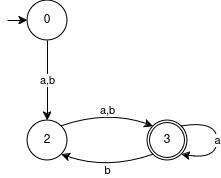
\includegraphics[scale=0.75]{MiniDEA2} 

\paragraph{(c)}
	Für diesen Automaten bleibt nach Durchführung des beschriebenen Tabellenfüllverfahrens eine Zelle ungefüllt. Dies ist der Nachweis, dass die Zustände 1 und 3 äquivalent zueinander sind und damit in der selben Äquivalenzklasse liegen.

	\includegraphics[scale=0.75]{Tabellenfüllverfahren4.png}		
	
	\begin{tabular}{c|c|c|l}
		\textbf{Zustandspaar} & \textbf{a} & \textbf{b} & \textbf{Erläuterung} \\
		\hline
		(2,0)                 & (1,3)      & (2,3)      & Eingabe b: (2,3) führt zu X0. Ergänze X1. \\
		\hline
		(3,1)                 & (3,3)      & (1,1)      & Kein Kreuz. \\
	\end{tabular}

	Der minimierte DEA besitzt nun noch einen Endzustand und kann folgendermaßen zusammengefasst werden:
	
	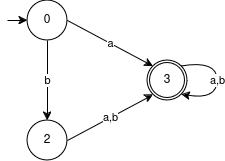
\includegraphics[scale=0.75]{MiniDEA3} 

